\documentclass[10pt, twocolumn, letterpaper]{article}
\usepackage{amsmath,amssymb,amsfonts}
\usepackage{lmodern}
\usepackage{graphicx}
\usepackage{cite}
\usepackage{geometry}
\geometry{margin=0.75in}
\usepackage{tabularx}
\usepackage{booktabs}

% Macros to simulate IEEEtran
\newcommand{\IEEEauthorblockN}[1]{\large\textbf{#1}\\}
\newcommand{\IEEEauthorblockA}[1]{\normalsize\textit{#1}\\}
\newcommand{\IEEEkeywords}{\textbf{\textit{Index Terms---}}}
\newenvironment{IEEEkeywords_env}{\vspace{1em}\noindent\IEEEkeywords}{}

\title{\vspace{-0.5in}\Large\textbf{Performance Evaluation of the Backpressure Collection Protocol (BCP) over Static Wireless Networks}}

\author{
\IEEEauthorblockN{Chin-Wei Huang}
\IEEEauthorblockA{Ming Hsieh Department of Electrical and Computer Engineering} 
\IEEEauthorblockA{University of Southern California}\\
\IEEEauthorblockA{Los Angeles, California}
}
\date{}

\begin{document}

\maketitle

\begin{abstract}
This paper presents the implementation and evaluation of the Backpressure Collection Protocol (BCP) over a static wireless network using the PyWiSim simulator. Motivated by the need for efficient dynamic routing without explicit path maintenance, the study contrasts BCP against a naive Random Walk baseline to highlight backpressure's routing efficiency. Furthermore, it investigates the critical impact of queue management by comparing Last-In-First-Out (LIFO) and First-In-First-Out (FIFO) scheduling mechanisms. By analyzing queue backlog states, we empirically justify why LIFO scheduling achieves significantly lower delay for delivered packets in backpressure environments. An extensive numerical evaluation of the network's stability region reveals that BCP sustains a maximum throughput capacity of approximately 0.85 packets per second, drastically outperforming the Random Walk baseline (0.18 packets per second). The simulation code and experimental data are provided in a public repository for full reproducibility.
\end{abstract}

\begin{IEEEkeywords_env}
Backpressure routing, BCP, wireless networks, LIFO scheduling, PyWiSim, Stability Region.
\end{IEEEkeywords_env}

\section{Introduction}
Routing in wireless sensor and ad-hoc networks faces unique challenges due to dynamic link conditions, interference, and fluctuating topologies. Traditional routing protocols establish explicit paths, which can become brittle and incur significant overhead when links fail. To address this, the Backpressure Collection Protocol (BCP) was introduced as a dynamic routing algorithm that makes per-packet routing and scheduling decisions based on local queue differentials and link state information \cite{b1}. By forwarding packets to neighboring nodes that offer the highest positive queue gradient, BCP inherently mitigates congestion and dynamically routes around poor link conditions without requiring end-to-end path discovery.

The motivation of this research is to explicitly evaluate the practical performance of BCP in a static wireless mesh network, focusing on the interplay between the protocol's routing gradients and queue scheduling disciplines. Specifically, we aim to demonstrate why traditional First-In-First-Out (FIFO) queue management performs poorly in backpressure routing and why Last-In-First-Out (LIFO) is strictly necessary to minimize delivery delay. 

Conducted as a final research project for EE 597 at the University of Southern California \cite{b2}, this work implements BCP and a Random Walk baseline over the PyWiSim simulation framework. We define a rigorous system model and evaluate both stability limits and delay distributions, providing a comprehensive empirical analysis of backpressure dynamics.

\section{System Model}
To evaluate the protocol, we define a time-slotted wireless network model characterized by specific queuing and arrival dynamics.

\subsection{Network and Channel Model}
The system is modeled as a static wireless mesh network where nodes are distributed in a geometric coordinate plane. Time is slotted, with a fixed time slot length of $1$ second. The wireless medium supports a fixed link rate of exactly $1$ packet per time slot. The channel exhibits path loss, resulting in a distance-dependent packet delivery probability that informs Expected Transmission Count (ETX) estimations.

\subsection{Queuing Dynamics}
Each node maintains an internal data queue of infinite capacity to buffer incoming packets. During each time slot, a node can transmit at most one packet to a neighboring node, provided the scheduling algorithm permits it. 

\subsection{Arrival Model}
We assume a deterministic arrival model for exogenous traffic. Packets are generated at a source node according to a specified arrival rate $\lambda$ (measured in packets/second). This is implemented by injecting packets uniformly and deterministically across the available time slots.\footnote{For example, an arrival rate of $\lambda = 0.2$ means exactly one exogenous packet arrives every 5 time slots. This ensures a strict deterministic arrival pattern rather than a memoryless Poisson process.}

\section{Protocol Description}
In our PyWiSim implementation, each node executes the protocol logic at every time slot. The wireless medium utilizes Carrier Sense Multiple Access (CSMA) for medium access control, which is natively implemented within the PyWiSim framework to handle collision avoidance and manage concurrent transmissions. Nodes periodically exchange their current queue sizes with neighbors via local broadcasts (simulated as accessible local state). 

\subsection{BCP Weight Calculation}
The scheduling decision in BCP is governed by a weight function that incorporates both the queue differential and a link penalty (ETX). For any node $i$ considering a transmission to a neighbor $j$, the link weight $W_{ij}$ is calculated as:
\begin{equation}
    W_{ij} = (Q_i - Q_j) - V \cdot \text{ETX}_{ij}
\end{equation}
where $Q_i$ and $Q_j$ represent the backlog sizes at nodes $i$ and $j$, respectively. The control parameter $V \ge 0$ dictates the strictness of the penalty for poor links; higher $V$ favors links with fewer expected retransmissions, while $V=0$ strictly follows the queue gradient. A node will transmit its packet to the neighbor $j^*$ that maximizes $W_{ij}$, provided that $W_{ij^*} > 0$. If no neighbor yields a strictly positive weight, the node retains its packet for that time slot.

\subsection{Random Walk Baseline}
To quantify the efficiency of BCP's gradient-based routing, we implemented a Random Walk protocol as a naive baseline. In this protocol, queue gradients and ETX penalties are completely ignored. Instead, if a node has a non-empty queue, it randomly selects one of its physical neighbors and attempts to forward the packet.

\section{Evaluation Setup}

\begin{figure}[htbp]
\centerline{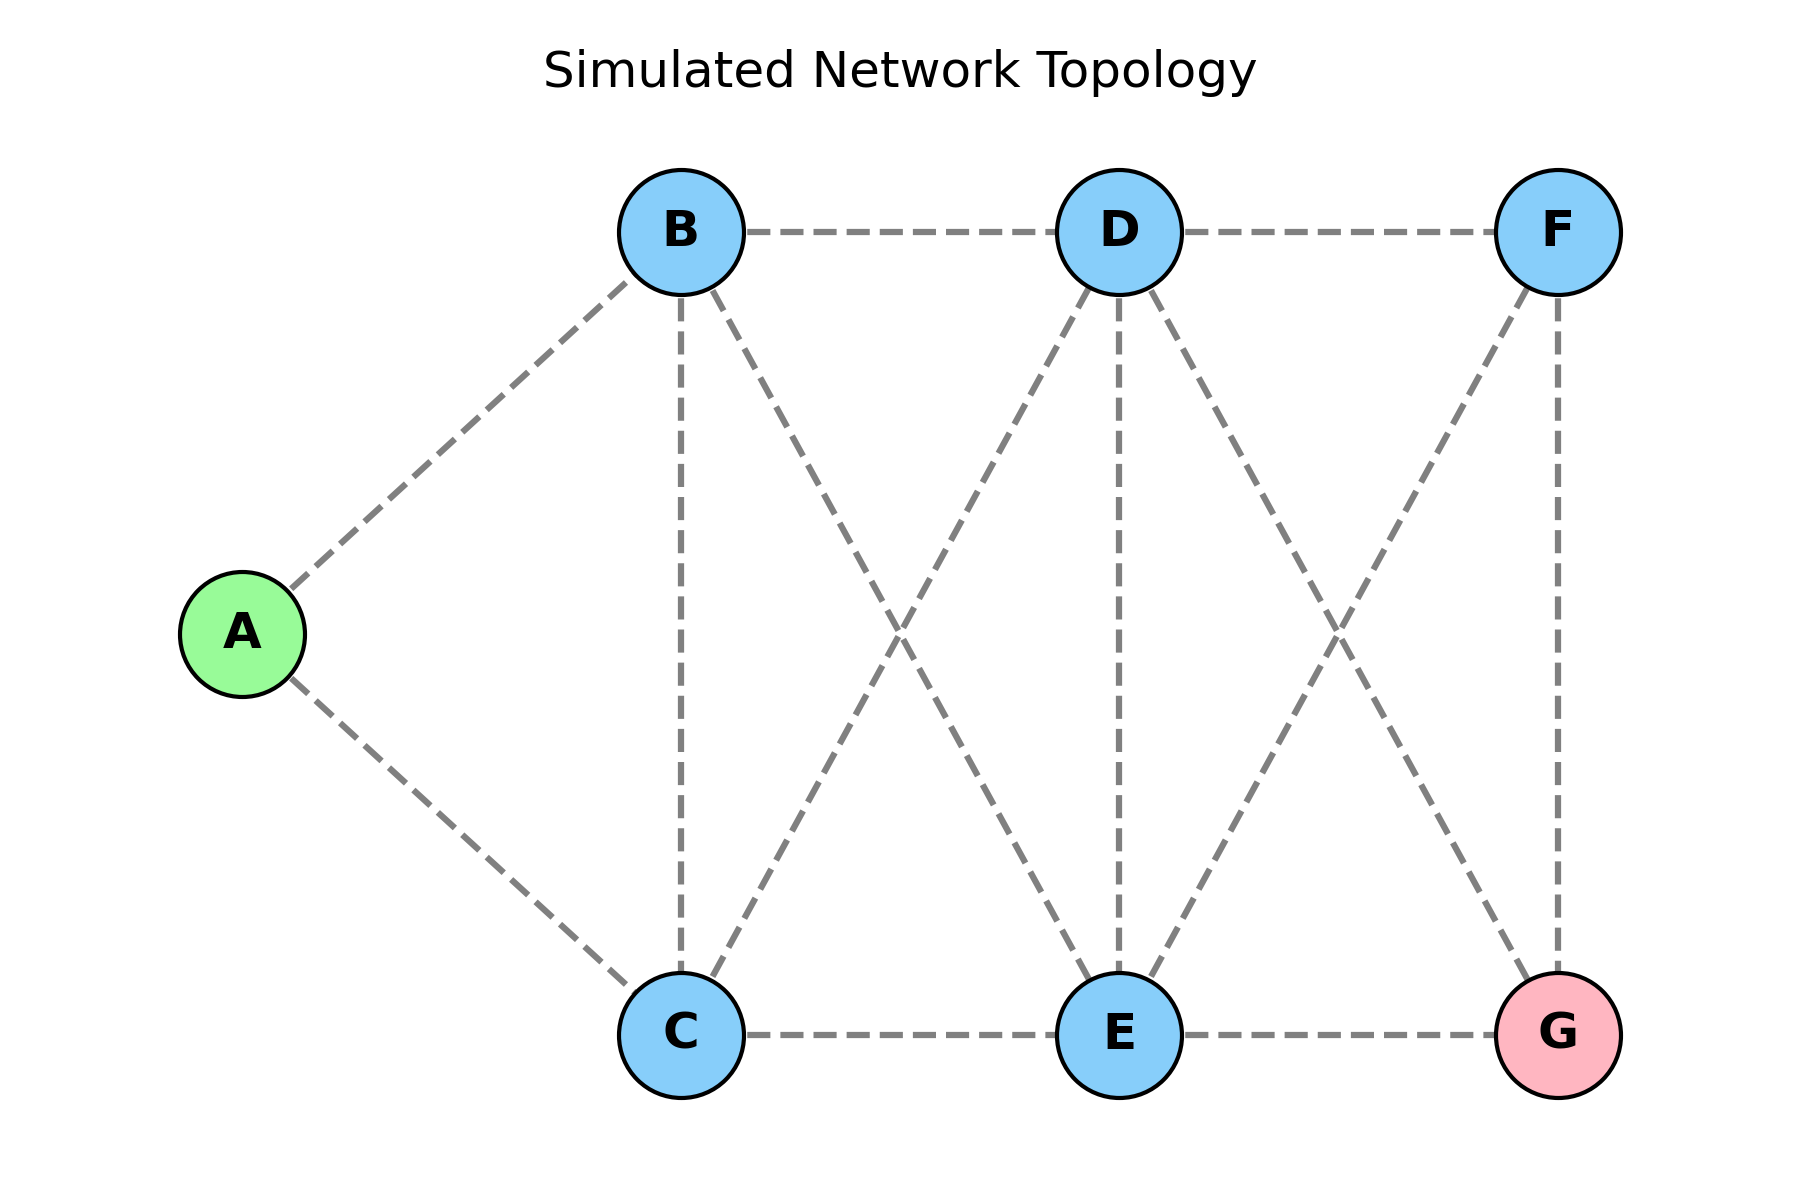
\includegraphics[width=0.85\linewidth]{topology.png}}
\caption{The 7-node static mesh network topology evaluated in PyWiSim. Node A serves as the traffic source, and Node G acts as the data sink.}
\label{fig_top}
\end{figure}

The protocols were evaluated using the PyWiSim framework over the 7-node topology depicted in Fig.~\ref{fig_top}. Node A acts as the singular traffic source, and Node G acts as the singular data sink. 

Two distinct simulation tests were conducted to evaluate different performance metrics:
\begin{itemize}
    \item \textbf{Test 1 (Queue State Analysis):} A short-duration simulation consisting of the first 20 seconds with 20 exogenous packets (arrival rate $\lambda = 1.0$) and 5 more seconds with no exogenous packets. This test aims to isolate the internal queue states and trace individual packet delays to observe the exact effect of LIFO versus FIFO scheduling.
    \item \textbf{Test 2 (Stability Region Analysis):} A long-duration simulation generating 10,080 packets per run. The arrival rate $\lambda$ was swept from 0.2 to 2.0 packets/second to empirically determine the maximum sustainable throughput (the stability region) and observe the corresponding scaling of packet delay.
\end{itemize}

\section{Results and Analysis}

\subsection{Queue State and LIFO Justification}
Traditional queue management relies on FIFO scheduling. However, backpressure routing fundamentally requires a "gradient" of backlogged packets across the network to push data toward the sink. If FIFO is used, newly arrived packets must wait behind the existing gradient, resulting in severe delay.

\begin{table}[htbp]
\caption{End-of-Simulation Queue States (20 pkts)}
\vspace{0.5em}
\begin{center}
\renewcommand{\arraystretch}{1.2}
\begin{tabularx}{\linewidth}{|c|c|X|X|}
\hline
\textbf{Node} & \textbf{Size} & \textbf{FIFO Content} & \textbf{LIFO Content} \\
\hline
A & 3 & Pkts 17--19 & Pkts 0, 3, 8 \\
\hline
B & 2 & Pkts 14, 16 & Pkts 1, 6 \\
\hline
C & 2 & Pkts 13, 15 & Pkts 2, 7 \\
\hline
D & 1 & Pkt 12 & Pkt 4 \\
\hline
E & 1 & Pkt 11 & Pkt 5 \\
\hline
F & 1 & Pkt 0 & Pkt 9 \\
\hline
G & 0 & Older Arrived & Newer Arrived \\
\hline
\end{tabularx}
\label{tab1}
\end{center}
\end{table}

To demonstrate this, we analyzed the final queue states of Test 1 (Table~\ref{tab1}). The backlog sizes across all intermediate nodes are strictly identical for both scheduling disciplines, perfectly illustrating the progressive routing gradient ($A=3 \rightarrow B,C=2 \rightarrow D,E,F=1 \rightarrow G=0$). However, the \textit{content} of these queues drastically differs:
\begin{itemize}
    \item \textbf{Under FIFO}: Older packets successfully reach the sink, but newer packets (e.g., Pkts 11--19) remain trapped in the queues of intermediate nodes (A--E) to form the necessary gradient.
    \item \textbf{Under LIFO}: Older packets (e.g., Pkts 0--9) are retained across all intermediate nodes (A--F) to establish a static gradient. This allows newer packets to "surf" over the established gradient and rapidly reach the sink.
\end{itemize}

This queue state analysis empirically proves that LIFO scheduling is essential for backpressure networks, as it minimizes delivery delay by utilizing older packets merely as the structural gradient.

\subsection{Throughput and Stability Region}
Fig.~\ref{fig_thr} details the results of Test 2. We observe that BCP (both LIFO and FIFO) scales linearly with the arrival rate until it reaches a stability limit of approximately \textbf{0.85 packets/second}. This capacity ceiling is a direct consequence of the specific network topology, the shared wireless nature of the medium, and the CSMA mechanism, which collectively restrict the number of concurrent non-interfering routes and limit their effective transmission rates. Beyond this threshold, the network is saturated. In stark contrast, the naive Random Walk baseline saturates almost immediately, capping at a maximum throughput of roughly \textbf{0.18 packets/second} due to highly inefficient, undirected ping-ponging of packets between nodes.

\begin{figure}[htbp]
\centerline{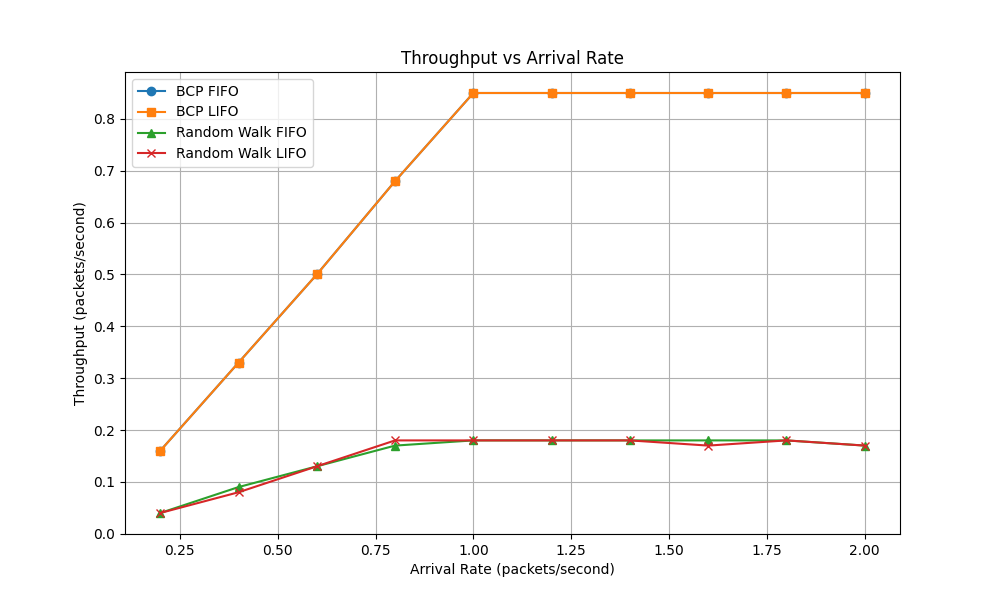
\includegraphics[width=\linewidth]{throughput_comparison.png}}
\caption{Network throughput versus packet arrival rate. BCP sustains a capacity of 0.85 pkt/s, far outperforming the Random Walk baseline.}
\label{fig_thr}
\end{figure}

\subsection{Packet Delay Scaling}
The choice of queue scheduling profoundly impacts the delay under varying loads, as shown in Fig.~\ref{fig_del}. 

\begin{figure}[htbp]
\centerline{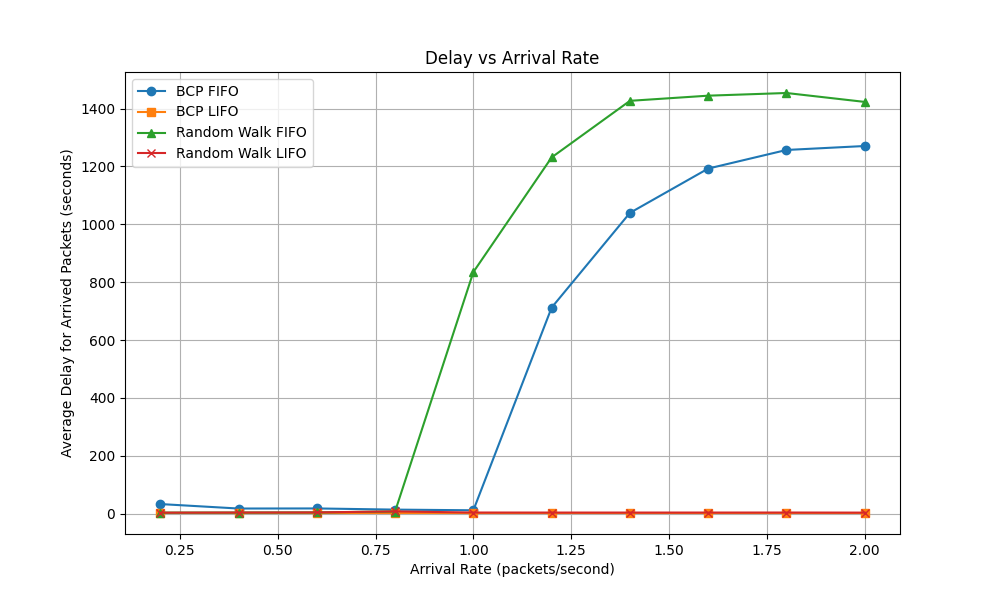
\includegraphics[width=\linewidth]{delay_comparison_arr.png}}
\caption{Average delay for successfully delivered packets versus arrival rate.}
\label{fig_del}
\end{figure}

For BCP-LIFO, the delay for delivered packets remains remarkably constant at \textbf{2.01 seconds}, even when the arrival rate pushes the network past its capacity boundary (0.85 pkt/s). Conversely, BCP-FIFO sees its delivery delay skyrocket to over 1,200 seconds once the network is saturated, as packets must slowly migrate through massive queues. 

\section{Conclusion}
This project successfully implemented and evaluated the Backpressure Collection Protocol against a Random Walk baseline in a simulated wireless environment. The results clearly outline BCP's superior stability region (0.85 pkt/s vs 0.18 pkt/s). Through queue backlog analysis, we provided concrete empirical justification for LIFO scheduling in backpressure networks. 

While BCP-LIFO guarantees a remarkably low delivery delay by maintaining routing gradients using older packets, a notable limitation of this study is the assumption of a static topology and a single traffic flow. Future work could explore multi-commodity flows and the impact of dynamic node mobility on gradient stability.

\section*{Code Repository}
The complete PyWiSim simulation code, protocol implementations, and raw experimental data are publicly accessible at: \texttt{https://github.com/ChinWeiHuang/EE597-BCP-PyWiSim}

\begin{thebibliography}{00}
\bibitem{b1} S. Moeller, A. Sridharan, B. Krishnamachari, and O. Gnawali, ``Routing without routes: the backpressure collection protocol,'' in \textit{Proceedings of the 9th ACM/IEEE International Conference on Information Processing in Sensor Networks (IPSN)}, 2010, pp. 279--290.
\bibitem{b2} B. Krishnamachari, ``EE 597: Wireless Networks,'' Course Materials, University of Southern California, 2026.
\end{thebibliography}

\end{document}
